\section{实验}
\label{sec:experiments}

在具有挑战性的nuScenes \cite{caesar2020nuscenes} 数据集上进行大量实验，验证了本文方法的有效性和优越性。公正地，将对全栈任务中的每个任务性能进行评估，与先前方法（无论是否为端到端方式）进行比较。总之，本节实验使用三种不同配置的SparseAD：SparseAD-B和SparseAD-L（仅使用图像输入），以及SparseAD-BR（使用雷达点云和图像多模态输入）。SparseAD-B和SparseAD-BR均使用V2-99\cite{lee2020centermask} 作为图像骨干网络，输入图像分辨率为 $1600\times640$。SparseAD-L进一步使用ViT-Large\cite{dosovitskiy2020image} 作为图像骨干网络，输入图像分辨率为 $1600\times800$。实验更多细节详见 \cref{appendix-exps}。

\subsection{综合结果}
\begin{table*}[t]
	\caption{SparseAD与当前最优全任务端到端自动驾驶方法在多任务性能上的综合比较。Ped.：人行横道，Div：分隔线，T.Mem：训练内存占用。}
	\begin{center}
	\tiny
	% \renewcommand\arraystretch{1.5}
	\vspace{-10pt}
	\resizebox{1\textwidth}{!}
	{
	\begin{tabular}{l|c|cc|cc|cc|ccc|cc|ccc}
	\toprule
	\multirow{2}{*}{方法} &
	\multirow{2}{*}{模态} &
	\multicolumn{2}{c|}{检测} &
	\multicolumn{2}{c|}{跟踪} &
	\multicolumn{2}{c|}{在线建图} &
	\multicolumn{3}{c|}{运动预测} &
	\multicolumn{2}{c}{规划 } &
	\multicolumn{3}{c}{效率} \\
	&& mAP$\uparrow$ & NDS$\uparrow$ & AMOTA$\uparrow$&Recall$\uparrow$ &IoU-Ped.$\uparrow$ & Iou-Div.$\uparrow$& minADE$\downarrow$&minFDE$\downarrow$&MR$\downarrow$ &平均L2$\downarrow$ &平均碰撞率$\downarrow$ & 参数量 & 训练内存 & FPS\\
	\midrule
	UniAD\cite{hu2023planning}&C&0.380& 0.499& 0.359& 0.467&0.138&0.257&1.17& 1.65& 0.205& 1.03 &0.31&124&50.0&1.8\\
	\midrule
	SparseAD-B&C& 0.475& 0.578& 0.530& 0.608 &0.164&0.288& 0.83& 1.58& 0.187& 0.35& 0.09&124&17.5&3.5\\
	SparseAD-BR&C+R&0.480& 0.579 & 0.534 &0.635&0.165&\textbf{0.289}&0.81& 1.55 &0.183 &\textbf{0.34}& 0.08&125&17.6&3.5\\
	SparseAD-L&C&\textbf{0.536}& \textbf{0.625} & \textbf{0.606}& \textbf{0.706}&\textbf{0.168}&0.278&\textbf{0.74}& \textbf{1.46}& \textbf{0.169}& \textbf{0.34}& \textbf{0.06}&376&31.6&0.7\\
	\bottomrule
	\end{tabular}% }
	}
	\end{center}
	\label{tab:joint-results}
	\end{table*}

如 \cref{tab:joint-results} 所示，\model 在所有任务上取得了更优异的性能，速度提升近 $\mathbf{1 \boldsymbol{\times}}$，内存占用相比UniAD \cite{hu2023planning} 仅为 \textbf{35\%}，UniAD具备全栈驾驶任务能力且在端到端自动驾驶领域具有深远影响。

具体而言，仅使用多视角相机输入，将mAP、NDS、AMOTA、召回率等指标分别提升至 \textbf{47.5\%}、\textbf{57.8\%}、\textbf{53\%}、\textbf{60.8\%}，这再次明显证明了稀疏架构在障碍物感知方面的优越性。对于在线建图，\model 相比使用BEV特征进行密集场景表示的UniAD \cite{hu2023planning} 也获得了更好的性能。在运动预测和规划任务上，\model 同样取得了显著更优的结果，minADE、平均L2误差和碰撞率分别大幅降低至 \textbf{0.83m}、\textbf{0.35m} 和 \textbf{0.09\%}。本文认为这既得益于上游感知任务的优越性能，也归功于运动规划器的合理设计。

此外，通过引入多视角相机和雷达的多模态传感器输入，几乎无需额外的训练和计算成本，有效提升了\model 的性能。同时，借助ViT-Large\cite{dosovitskiy2020image} 先进骨干网络，综合性能进一步提升，有力地证明了稀疏查询中心范式通过扩展规模以获得更优性能的潜力。

\subsection{多任务结果}
\begin{table}[t]
\centering
\caption{nuScenes \texttt{val} 数据集上的3D检测和3D多目标跟踪结果。"Tracking-only methods"指通过后处理关联进行跟踪的方法。"End-to-End Autonomous Driving Method"指具备自动驾驶全栈任务能力的方法。表中所有方法均在完整分辨率图像输入下进行评估。$^\dag$：通过官方开源代码复现的结果。-R：带雷达点云输入。}
\label{tab:det_tracking_val_set}
\tiny
\resizebox{\textwidth}{!}{
% {
\setlength{\tabcolsep}{3.5pt}
\begin{tabular}{l|c|c|ccc|l|cccc}

\toprule
\textbf{方法}&  \textbf{mAP}$\uparrow$  &\textbf{NDS}$\uparrow$  & \textbf{mATE}$\downarrow$  &\textbf{mAOE}$\downarrow$   &\textbf{mAVE}$\downarrow$ & \textbf{方法}& \textbf{AMOTA}$\uparrow$  & \textbf{AMOTP}$\downarrow$ & \textbf{RECALL}$\uparrow$ & \textbf{IDS}$\downarrow$\\
\midrule
\multicolumn{5}{l}{\textit{纯检测方法}}&&\multicolumn{5}{l}{\textit{纯跟踪方法}}\\
\midrule
% ResNet101
StreamPETR\cite{wang2023exploring}                            &0.504  &0.592  &0.569    &0.315  &0.257  &DEFT\cite{chaabane2021deft} & 0.201 & - & - & -\\
SOLOFusion\cite{park2022time}                & 0.483 & 0.582 & \textbf{0.503}  & 0.381 & 0.246 &QD3DT\cite{hu2022monocular} & 0.242 & 1.518 & 0.399  & 5646 \\
BEVDepth\cite{li2023bevdepth}                         & 0.412 & 0.535 & 0.565  & 0.358 & 0.331 &TripletTrack~\cite{marinello2022triplettrack} & 0.285 & 1.485 &-  & - \\ % PETR Table 1
BEVFormer \cite{li2022bevformer}                  & 0.416 & 0.517 & 0.673  & 0.372 & 0.394 & CC-3DT$^*$~\cite{fischer2022cc} & 0.429 & 1.257 & 0.534 & 2219 \\
Sparse4D\cite{lin2022sparse4d}                 & 0.436 & 0.541 & 0.633  & 0.363 & 0.317  &QTrack\cite{yang2022quality} &0.511& \underline{1.090}& 0.585 & 1144\\
SRCN3D\cite{shi2022srcn3d}& 0.396& 0.475& 0.737& \underline{0.278}& 0.728& SRCN3D\cite{shi2022srcn3d} &0.439 &1.280& 0.545&-
\\

\midrule
\multicolumn{7}{l}{\textit{端到端多目标跟踪方法}}\\
\midrule
MUTR3D\cite{zhang2022mutr3d}  &-&-&-&-&-& MUTR3D\cite{zhang2022mutr3d} &0.294& 1.498& 0.427 &  3822 \\
PF-Track$^\dag$\cite{pang2023standing} &	0.382& 0.486&	0.702&	0.430&	0.463 &PF-Track$^\dag$\cite{pang2023standing} & {0.479} & {1.227} & {0.590}  & \textbf{181}\\
Sparse4Dv3\cite{lin2023sparse4d} &\textbf{0.537} &\underline{0.623}&\underline{0.511} & 0.306 &\textbf{0.194} & Sparse4Dv3\cite{lin2023sparse4d} &\underline{0.567}& 1.027 & \underline{0.658}& 557\\
\midrule
\multicolumn{7}{l}{\textit{端到端自动驾驶方法}}\\
\midrule
UniAD\cite{hu2023planning} &0.380&0.499&0.684	&	0.383	&0.378& UniAD\cite{hu2023planning} &0.359 &1.320 &0.467 &906\\
\rowcolor[gray]{.9}  \model-B& 0.475 & 0.578&0.556	&	0.295&	0.288	& \model-B & 0.530	& 1.087&	0.608 & 297\\
\rowcolor[gray]{.9}  \model-BR& 0.480 & 0.579 &0.554	&	0.316&	0.273	& \model-BR & 0.534	& 1.077&	0.635 & 277\\
\rowcolor[gray]{.9}  \model-L& \underline{0.536} & \textbf{0.625} &0.531	&	\textbf{0.219}&	\underline{0.230}	& \model-L & \textbf{0.606}	& \textbf{0.933}&	\textbf{0.706} & \underline{251}\\
\bottomrule
\end{tabular}}
\vspace{-0.25cm}
\end{table}

\paragraph{\textbf{障碍物感知。}}
在 \cref{tab:det_tracking_val_set} 中将\model 与nuScenes \texttt{val} 集上的其他方法进行了检测和跟踪性能对比。显然，\model-B在大多数流行的纯检测、纯跟踪和端到端多目标跟踪方法 \cite{li2023bevdepth, li2022bevformer, pang2023standing,zhang2022mutr3d} 中表现最优，同时在相应任务上与SOTA方法（如StreamPETR\cite{wang2023exploring}、QTrack\cite{yang2022quality}）保持可比性能。通过先进骨干网络的扩展，\model-Large在整体上取得了更优性能，mAP达到 \textbf{53.6\%}，NDS达到 \textbf{62.5\%}，AMOTA达到 \textbf{60.6\%}，整体优于先前SOTA方法Sparse4Dv3 \cite{lin2023sparse4d}。

\begin{table}[t]
		\caption{与在线建图方法的性能比较。结果在 $[1.0m, 1.5m, 2.0m]$ 阈值下评估。$\ddag$：通过官方开源代码复现。$\dag$：基于\model 中规划模块的需求，将\textit{边界}进一步划分为\textit{道路段}和\textit{车道}分别评估。$*$：骨干网络和稀疏感知模块的成本。-R：带雷达点云输入。}
	        \vspace{-10pt}
	        % \scriptsize
	        \tiny
		\begin{center}
			% \resizebox{1.0\textwidth}{!}
	            {
				\begin{tabular}{l|p{1.3cm}<{\centering}p{1.3cm}<{\centering}p{2cm}<{\centering}p{1cm}<{\centering}p{3.0cm}<{\centering}}
					\toprule
					方法 & \textbf{分隔线}$\uparrow$& \textbf{人行横道}$\uparrow$ & \textbf{边界}$\uparrow$ & mAP$\uparrow$ & 训练内存(GB)$\downarrow$\\
	                \midrule
	                \multicolumn{6}{l}{\textit{纯在线建图方法}}\\
	                \midrule
					HDMapNet$^\ddag$ \cite{li2022hdmapnet} & 18.0 & 23.1 & 33.5 & 24.9  & 21.1\\
					VectorMapNet$^\ddag$ \cite{liu2023vectormapnet}  & 39.8 &  38.7 & 19.9 & 32.8 &16.4\\
					MapTR$^\ddag$ \cite{liao2022maptr}  & 17.9 &  36.9 & 1.8 & 18.9 & 20.0\\
				  StreamMapNet$^\ddag$ \cite{yuan2024streammapnet} & 55.5 &  59.7 & 46.7 & 54.0 &23.2\\
					\midrule
	                \multicolumn{6}{l}{\textit{端到端多目标跟踪方法}}\\
	                \midrule
					\rowcolor[gray]{.9} {SparseAD-B}  & {37.3}& {45.2} & {29.2/25}$^\dag$ & {34.2} & \textbf{6.9}$^*$\\
	                    \rowcolor[gray]{.9} {SparseAD-BR}  & {38.4}& {44.5} & {29.4/24.7}$^\dag$ & {34.2} & 7.1$^*$\\
	                    \rowcolor[gray]{.9} {SparseAD-L}  & {37.6}& {46.7} & {30/24.8}$^\dag$ & {34.8} & 19.3$^*$\\
	                \bottomrule
				\end{tabular}
			}
		\end{center}
		\label{tab:map-nuscenes-val}
	         \vspace{-10pt}
	\end{table}

\paragraph{\textbf{在线建图。}} 在 \cref{tab:map-nuscenes-val} 中展示了\model 与先前其他方法在nuScenes \texttt{val} 集上的在线建图对比结果。需要指出的是，将\textit{边界}划分为\textit{道路段}和\textit{车道}分别评估，并将范围从通常的 $60m \times 30m$ 扩展到 $102.4m \times 102.4m$，以与障碍物感知保持一致，满足规划需求。在不失公平性的前提下，\model 以稀疏端到端方式在无需任何密集BEV表示的情况下取得了 \textbf{34.2\%} 的mAP，优于大多数先前流行方法（如HDMapNet \cite{li2022hdmapnet}、VectorMapNet \cite{liu2023vectormapnet} 和MapTR \cite{liao2022maptr}），在性能和训练成本方面均具有明显优势。虽然性能落后于StreamMapNet \cite{yuan2024streammapnet}，但本文证明了可以在统一的稀疏方式下完成在线建图而无需任何密集BEV表示，这对以显著更低成本进行端到端自动驾驶的实际部署具有重要意义。诚然，如何有效利用其他模态（如雷达）的有用信息仍然是值得进一步探索的任务。本文认为稀疏方式下仍有很大的探索空间。

\paragraph{\textbf{运动预测。}} 在 \cref{tab:motion_vip3d_val_set} 中展示了运动预测的对比结果，其中指标与VIP3D \cite{gu2023vip3d} 一致。\model 在所有端到端方法 \cite{liang2020pnpnet, gu2023vip3d, hu2023planning} 中取得了最优性能，最低minADE为 \textbf{0.83m}，minFDE为 \textbf{1.58m}，缺失率为 \textbf{18.7\%}，EPA最高达 \textbf{0.308}，具有巨大优势。此外，得益于稀疏查询中心范式的高效性和可扩展性，\model 能够高效扩展到更多模态并从先进骨干网络中受益，进一步显著提升了预测性能。

\begin{table}[t]

    \centering
    % \scriptsize
    \caption{SparseAD在nuScenes \texttt{val} 数据集上的运动规划器综合性能。-R：带雷达点云输入。}
    \vspace{-5pt}
    \begin{subtable}[h]{0.45\textwidth}
    \tiny

    {
    \begin{tabular}{l|cccc}
			\toprule
			方法 & minADE$\downarrow$ & minFDE$\downarrow$ & MR$\downarrow$ & EPA$\uparrow$ \\
			\midrule
            Traditional\cite{gu2023vip3d} &2.06&3.02&0.277&0.209\\
			PnPNet~\cite{liang2020pnpnet} & 2.04 & 3.03 & 0.271 & 0.213 \\
			ViP3D~\cite{gu2023vip3d} & 2.03 & 2.90 & 0.239 & 0.236 \\
			{UniAD}\dag~\cite{hu2023planning} & 1.17&	1.65&	0.205&	0.205 \\
	        \midrule
	        \rowcolor[gray]{.9} \model-B & 0.83&	1.58	&0.187& 0.308\\
	        \rowcolor[gray]{.9} \model-BR & 0.81&	1.55&	0.183& \textbf{0.316}\\
	         \rowcolor[gray]{.9} \model-L &\textbf{0.74}	&\textbf{1.46}&	\textbf{0.169}& 0.292\\
			\bottomrule
		\end{tabular}
	        }
	        \caption{与先前基于视觉的端到端方法在ViP3D\cite{gu2023vip3d}基准上的运动预测性能对比。$\dag$：使用官方检查点\cite{hu2023planning}评估。}
		\label{tab:motion_vip3d_val_set}
    \end{subtable}
    \hfill
    \begin{subtable}[h]{0.50\textwidth}
    \tiny

    \begin{tabular}{l|cccc|cccc}
    \toprule
    \multirow{2}{*}{方法} &
    \multicolumn{4}{c|}{L2 (m) $\downarrow$} &
    \multicolumn{4}{c|}{碰撞率 (\%) $\downarrow$} \\

    & 1s & 2s & 3s & 平均 & 1s & 2s & 3s & 平均 \\
    \midrule
    EO$^\dagger$~\cite{khurana2022differentiable}& 0.67 & 1.36 & 2.78 & 1.60 & 0.04 & 0.09 & 0.88 & 0.33   \\
    \midrule
    ST-P3~\cite{hu2022st}& 1.33 & 2.11 & 2.90 & 2.11 & 0.23 & 0.62 & 1.27 & 0.71  \\
    UniAD~\cite{hu2023planning} & 0.48 & 0.96 & 1.65 & 1.03 & 0.05 & 0.17 & 0.71 & 0.31  \\
    VAD~\cite{jiang2023vad} & 0.17 & 0.34 & 0.60 & 0.37 & 0.07 & 0.10 & 0.24 & 0.14  \\
    \midrule
    \rowcolor[gray]{.9}  \model-B&\textbf{0.15}&\textbf{0.31}&0.57&0.35 &	\textbf{0.00}&0.06&0.21&0.09\\
    \rowcolor[gray]{.9}  \model-BR&0\textbf{.15}&\textbf{0.31}&\textbf{0.56}&\textbf{0.34}&	\textbf{0.00}&0.06&0.19&0.08\\
    \rowcolor[gray]{.9}  \model-L&\textbf{0.15}&\textbf{0.31}&\textbf{0.56}&\textbf{0.34}&	\textbf{0.00}&\textbf{0.04}&\textbf{0.15}&\textbf{0.06}\\
    \bottomrule
    \end{tabular}
    \caption{nuScenes \texttt{val} 数据集上的开环规划性能。带 \dag 标记为基于激光雷达的方法。}
    \label{tab:planning_val_set}
    \end{subtable}
    \vspace{-20pt}
\end{table}

\paragraph{\textbf{规划。}} 规划结果在 \cref{tab:planning_val_set} 中呈现。得益于上游感知模块和运动规划器的优越设计，\model 的所有版本在nuScenes \texttt{val} 数据集上均达到了当前最优水平。具体而言，\model-B与包括UniAD\cite{hu2023planning} 和VAD\cite{jiang2023vad} 在内的所有其他方法相比，取得了最低的平均L2误差和碰撞率，证明了本文方法和架构的优越性。与障碍物感知和运动预测等上游任务类似，\model 通过引入雷达或更强大的骨干网络获得了进一步改进。

\subsection{消融实验}

\begin{table*}[t]
	\caption{稀疏感知模块设计的消融实验。"Det. Mem."表示检测场景级记忆；"Map. Mem."表示地图场景级记忆；"Two-L. M. U."表示两层级记忆更新；"TQeury Aug."表示跟踪查询增强。}
	\begin{center}
	\tiny
	\vspace{-10pt}
	\resizebox{0.9\textwidth}{!}
	{
	\begin{tabular}{l|cccc|cc|ccc|c}
	\toprule
	\multirow{2}{*}{编号} &
	\multirow{2}{*}{\makecell{检测\\记忆}} &
	\multirow{2}{*}{\makecell{建图\\记忆}} &
	\multirow{2}{*}{\makecell{两层级\\记忆更新}} &
	\multirow{2}{*}{\makecell{跟踪查询\\增强}} &
	\multicolumn{2}{c|}{检测} &
	\multicolumn{3}{c|}{跟踪} &
	{建图} \\

	&&&& & mAP & NDS & AMOTA & AMOTP & Recall  & mAP  \\
	\midrule
	1& & & & & 0.4227	&0.5326	&0.443	&1.301&	0.538	&0.311\\
	2&\Checkmark & & & & 0.4261&	0.5451&	0.42&	1.301	&0.525	&0.317\\
	3&\Checkmark &\Checkmark & & & 0.4201&0.5414&0.415&1.316&0.513& 0.331\\
	4&\Checkmark &\Checkmark &\Checkmark & & 0.4294&	0.5457&	0.439&	1.272&	0.535	&	\textbf{0.337}\\
	5&\Checkmark &\Checkmark &\Checkmark &\Checkmark  &\textbf{0.4537}&	\textbf{0.5634}&	\textbf{0.472}&	\textbf{1.209}&	\textbf{0.58}	&	0.334\\
	\bottomrule
	\end{tabular}% }
	}
	\end{center}
	\label{tab:perception-ablations}
\end{table*}

\paragraph{\textbf{感知设计的影响。}} 在 \cref{tab:perception-ablations} 中提供了稀疏感知模块的消融实验。实验结果表明，引入场景级记忆用于检测和建图可以有效提升相应任务的性能。然而，由于训练过程中不同查询的监督可能不稳定，跟踪性能略有下降。借助两层级记忆的更新策略和跟踪查询增强策略，不同查询的监督变得更加平衡，所有感知任务的性能进一步得到提升。

\label{abalation:perceptrion}

\begin{table*}[t]
	\caption{运动规划模块设计的消融实验。"MQI"表示运动查询初始化；"AMI"表示智能体-记忆交互；"KN"表示自车运动学约束；"EAR"表示自车-智能体关系约束。}
	\begin{center}
	\tiny
	\vspace{-10pt}
	\resizebox{0.9\textwidth}{!}
	{
	\begin{tabular}{l|cccc|ccc|cccc|cccc}
	\toprule
	\multirow{2}{*}{编号} &
	\multirow{2}{*}{\makecell{MQI}} &
	\multirow{2}{*}{\makecell{AMI}} &
	\multirow{2}{*}{\makecell{KN}} &
	\multirow{2}{*}{\makecell{EAR}} &

	\multicolumn{3}{c|}{预测} &
	\multicolumn{4}{c|}{规划L2(m)} &
	\multicolumn{4}{c|}{规划碰撞率(\%)} \\

	&&&& & minADE&	minFDE	&MR & 1s & 2s  & 3s&平均 & 1s & 2s  & 3s&平均\\
	\midrule
	1&\Checkmark&\Checkmark&\Checkmark&\Checkmark&0.876&	1.654&	0.193&	\textbf{0.35}&\textbf{0.69}&\textbf{\textbf{1.13}}&\textbf{0.72}&0.02& \textbf{0.22} & \textbf{\textbf{0.66}}&\textbf{0.30}\\
	2&&\Checkmark&\Checkmark&\Checkmark&0.867&	1.660&	0.203	&\textbf{0.35} & 0.70 & 1.14	& 0.73 & 0.05 & 0.29&0.75 & 0.36\\
	3&\Checkmark&&\Checkmark&\Checkmark& 0.870&1.646&	0.193	&0.39&0.76&1.23&0.79&	0.03&0.45&1.27&0.58\\
	4&\Checkmark&\Checkmark&&\Checkmark&0.866&	1.646&	0.197	&0.36&0.71&1.15&0.74&	\textbf{\textbf{0.01}}&0.28&0.84&0.38\\
	5&\Checkmark&\Checkmark&\Checkmark&&0.864&	1.646&0.197&	\textbf{0.35}&\textbf{0.69}&\textbf{1.13}&\textbf{0.72}	&0.03&0.23&0.70&0.32\\
	\bottomrule
	\end{tabular}% }
	}
	\end{center}
	\label{tab:motionpalnner-ablations}
\end{table*}

\paragraph{\textbf{运动规划设计的影响。}} 需要指出的是，在开环规划场景中，排除了自车状态输入以防止捷径学习 \cite{li2023ego}。如 \cref{tab:motionpalnner-ablations} 所示，缺少运动预测器中的任何策略或规划优化器中引入的约束时，规划性能均会不同程度下降，有力证明了本文方法的正确性和有效性。

\label{abalation:planning}

\subsection{定性结果}
\begin{figure}[tb]
  \centering
  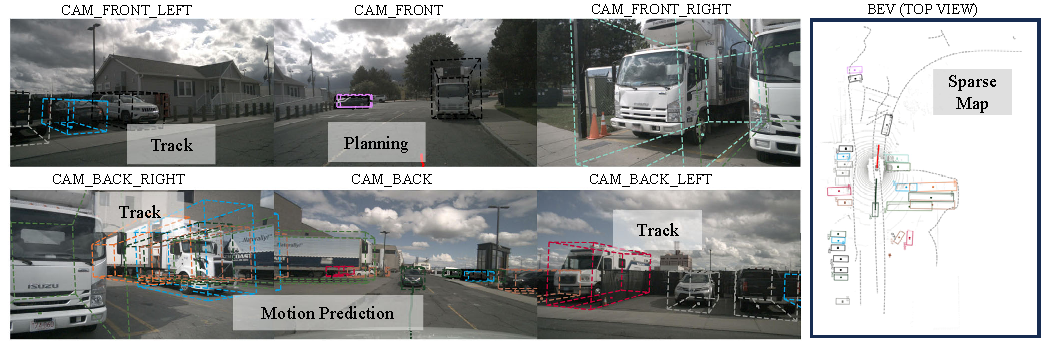
\includegraphics[width=1\linewidth]{Figures/Visualization-Figure}
  \caption{定性可视化。在环视图像和BEV中绘制所有任务的结果。每个智能体在图像和BEV中均以不同颜色的虚线边界框标记。地图元素的稀疏预测仅以灰色虚线在BEV中显示。分别选择运动预测的top-1模态和自车规划结果在图像和BEV上进行可视化。BEV中的激光雷达点云仅用于可视化，不作为模型输入。}
  \label{fig:vis}
\end{figure}

直观地，通过可视化展示所有任务的性能，如 \cref{fig:vis} 所示，其中具有挑战性的驾驶场景的特点是自车前后均有近距离智能体、路边存在大量潜在遮挡障碍物以及不规则的道路边界。即便如此，SparseAD仍然能够准确感知整个场景中的复杂元素，并提供合理且安全的规划轨迹。更多其他驾驶场景的可视化与分析详见 \cref{appendix-vis}。
